% Make nice A4 pages for print:
%\usepackage{pgfpages}
%\pgfpagesuselayout{resize to}[a4paper,border shrink=5mm,landscape]

\beamertemplatenavigationsymbolsempty

\setbeamertemplate{bibliography item}[text]

\usepackage[type={CC},modifier={by-sa},version={4.0}]{doclicense}

\usepackage[utf8]{inputenc}
\usepackage{hyperref}
\usepackage{breakurl}
\usepackage{graphicx}
\usepackage{pgfplots}
\usepackage{pgf}
\usepackage{tikz}
\usetikzlibrary{positioning}
\usetikzlibrary{arrows}
\usetikzlibrary{decorations.markings}
\usetikzlibrary{calc}
\usetikzlibrary{matrix}
\usetikzlibrary{shapes}
\usetikzlibrary{decorations.pathmorphing}
\usetikzlibrary{fit}
\usetikzlibrary{backgrounds}
\usetikzlibrary{plotmarks}
\usepackage{stmaryrd}
\usepackage{listings}
\usepackage{pdflscape}
\usepackage{perpage}
\usepackage{appendixnumberbeamer}

%\usepackage[thmmarks,amsmath,amsthm]{ntheorem} % already included in beamer
\usepackage{thm-restate}

\usepackage[sort&compress,numbers]{natbib}  % to be have \citet, \citeauthor, \citeyear

\MakePerPage{footnote}

\tikzstyle{o}=[r,ppBlue]
\tikzstyle{r}=[thick,rectangle,align=center]
\tikzstyle{t}=[r,ppTrans] %,font=\bfseries]
\tikzstyle{dd}=[densely dashed]
\tikzstyle{n}=[r,ppBlue]
\tikzstyle{p}=[r,ppRed]
\tikzstyle{ppRed}  =[draw=red,  fill=  red!20]
\tikzstyle{ppBlue} =[draw=blue, fill= blue!20]
\tikzstyle{ppGreen}=[draw=green,fill=green!20]
\tikzstyle{ppTrans}=[draw=none, fill=none]

\usetheme{Warsaw}

\useoutertheme[subsection=true]{smoothbars}
%\useoutertheme[subsection=false]{miniframes}

\definecolor{bblue}{HTML}{D7DF01}	% yellow-ish actually, for better black/white printing
\definecolor{rred}{HTML}{C0504D}
\definecolor{ggreen}{HTML}{9BBB59}
\definecolor{ppurple}{HTML}{9F4C7C}
\definecolor{lightgray}{rgb}{0.3,0.3,0.3}
\definecolor{lightergray}{rgb}{0.9,0.9,0.9}
\definecolor{UniBlue}{RGB}{83,121,170}

\DeclareTextFontCommand\textintro{\normalfont\bfseries\itshape} % nice!
\newcommand{\intro}[2][]
{%
	\textintro{#2}%
}
\newcommand{\empha}[2][]
{%
	\emph{#2}%
}

%\theoremstyle{plain}
\newcounter{reqcounter}
\newtheorem{requirement}[reqcounter]{Requirement}

%setbeamercolor{structure}{fg=violet}

\makeatletter
\def\th@task{%
    \normalfont % body font
    \setbeamercolor{block title example}{bg=orange,fg=white}
    \setbeamercolor{block body example}{bg=orange!20,fg=black}
    \def\inserttheoremblockenv{exampleblock}
  }
\makeatother

\theoremstyle{task}
\newtheorem{task}{Task}

\newenvironment{assignment}%
{%\setbeamercolor{background canvas}{bg=violet}%
%\setbeamercolor{structure}{fg=cyan!90!black}%
 \setbeamercolor{frametitle}{bg=orange,fg=white}
\begin{frame}}%
{\end{frame}}%

\AtBeginSection[]{
  \begin{frame}
  \vfill
  \centering
  \begin{beamercolorbox}[sep=8pt,center,shadow=true,rounded=true]{title}
    \usebeamerfont{title}\insertsectionhead\par%
  \end{beamercolorbox}
  \tableofcontents
  \vfill
  \end{frame}
}




\pgfplotsset{compat=1.14}
\author{Markus Raab}


\date{8.6.2018}

\begin{document}

\renewcommand{\enquote}[1]{\emph{``#1''}} % Cannot be done earlier

%%%%%%%%%%%%%%%%%%%%%%%%%%%%%%%
\begin{frame}
	\titlepage
	\doclicenseThis
\end{frame}

\begin{frame}
	\frametitle{Organization}
	Schedule:
	\begin{description}
		\item[8.6.2018:] lecture
		\item[15.6.2018:] last corrections of team exercise
		\item[22.6.2018:] oral test
	\end{description}
\end{frame}


\begin{frame}
	\frametitle{Popular Topics}
	\vspace{-0.5cm}
	\begin{multicols}{2}
	\begin{description}
	\color{gray}
	\item[4] validation
	\color{red}
	\item[4] user interface
	\color{gray}
	\item[3] tools (benefits?)
	\item[3] testability
	\item[3] complexity reduction (when conf. needed?)
	\item[3] architectural decisions
	\color{black}
	\item[2] Puppet
	\color{gray}
	\item[2] modularity
	\item[2] environment variables
	\item[2] documentation
	\color{red}
	\item[2] configuration specification
	\color{gray}
	\item[2] command-line args
	\item[2] code generation
	\item[1] variability
	\item[1] self-description
	\item[1] round-tripping
	\item[1] early detection
	\item[1] introspection
	\item[1] dependences
	\item[1] auto-detection
	\item[1] context-awareness
	\color{red}
	\item[1] administrators
	\end{description}
	\end{multicols}
\end{frame}


%%%%%%%%%%%%%%%%%%%%%%%%%%%%%%%%%%%%%%%%%% 
\section{Recapitulation}

\subsection{}

\begin{frame}
	\frametitle{Introspection (Recapitulation)}
	\begin{task}
	What is internal and external specification?
	What is introspection?
	\end{task}

	\pause
	\vspace{1em}

	\begin{itemize}
	\item \textit{internal}: within applications' source code
	\item \textit{introspection}: unified get/set access to (meta*)-key/values
	\item access via applications, CLI, GUI, web-UI, ...
	\item access via any programming language (similar to file systems)
	\item GUI, web-UI can semantically interpret metadata
	\item assemble modular parts (validation, logging, \dots)
	\item needed as communication between producers and consumers
	\item essential for \intro[no-futz computing]{no-futz computing}~\citet{holland2001nofutz}
	\end{itemize}
\end{frame}

\begin{frame}
	\frametitle{KeySet (Recapitulation)}

	The common data structure of Elektra:
	\vspace{1cm}

	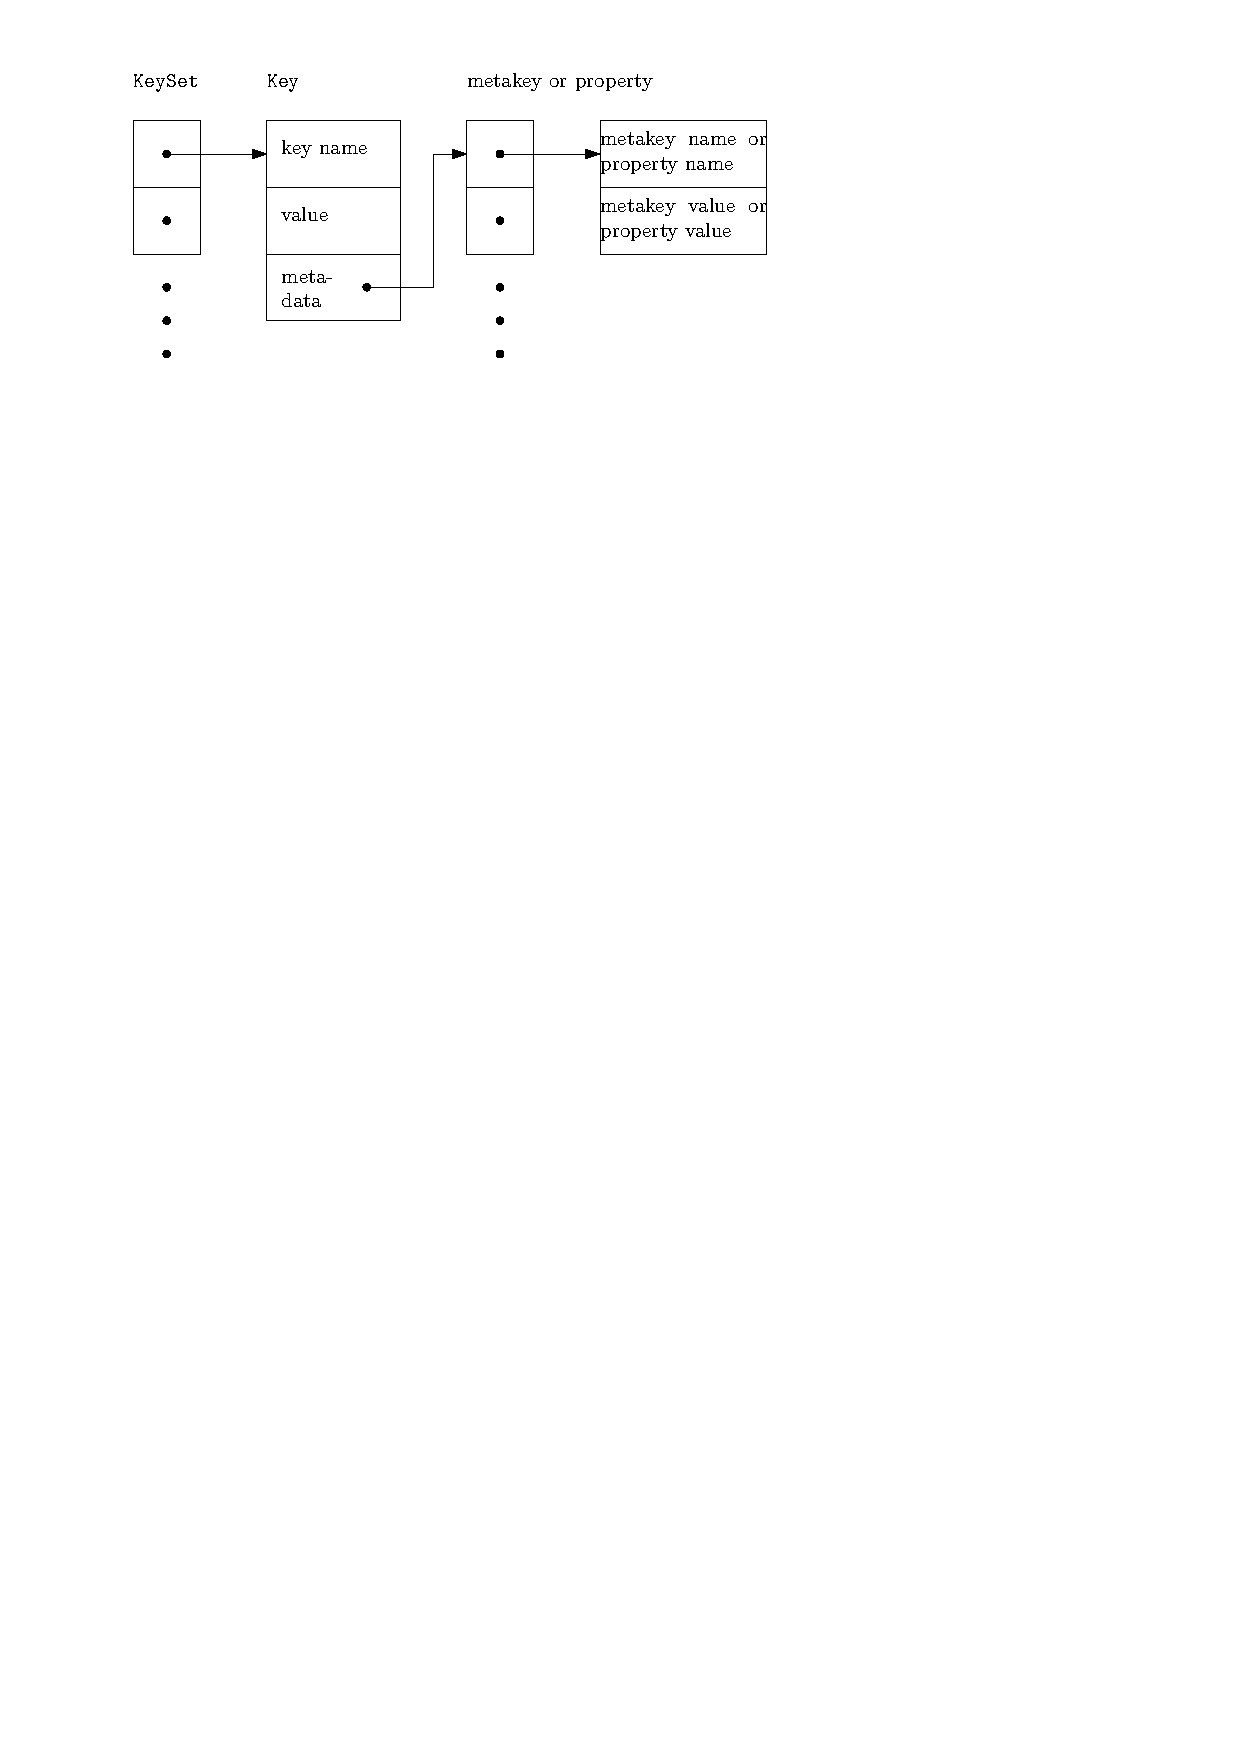
\includegraphics{keyset}
\end{frame}

\begin{frame}
	\frametitle{Testing (Recapitulation)}
	\begin{task}
	What do we want to test?
	\end{task}

	\pause

	\begin{itemize}
	\item That settings do what they should (devs and admins)
	\item That settings are properly validated (devs~\cite{xu2013blame})
	\item Regression tests (devs~\cite{qu2008configuration})
	\vspace{1em}
	\item Are all settings implemented? (devs)
	\item Are all settings used in tests? (devs)
	\item Are there unused settings in the code? (devs)
	\item Do the chosen settings work? (admins)
	\end{itemize}
\end{frame}

\begin{frame}
	\frametitle{Early detection (Recapitulation)}
	\begin{task}
	When do we want to detect misconfiguration?
	\end{task}

	\pause

	Phases when we can detect misconfigurations:
	\begin{itemize} %[<+-| alert@+>]
	\item Compilation stage in configuration management tool
	\item Writing configuration settings on nodes
	\item Starting applications (load-time)
	\item When configuration setting is actually used (run-time)
	\end{itemize}

	\pause[\thebeamerpauses]

	\begin{alertblock}{Problem}
	Earlier versus more context.
	\end{alertblock}
\end{frame}

\begin{frame}
	\frametitle{Notification (Recapitulation)}

	\begin{task}
	Why do we need notification?
	\end{task}

	\pause

	\begin{enumerate}
	\item to keep transient and persistent configuration settings always in sync~\cite{jin2014configurations}
	\item to avoid polling of configuration settings
	\item to better integrate into already existing mechanisms (main loops)\footnote{Is one of the main reasons why most framework already integrate configuration settings.}
	\end{enumerate}

	\ExecuteMetaData[../book/motivation.tex]{req-consistency}
\end{frame}

\begin{frame}
	\frametitle{Cascading (Recapitulation)}

	\begin{task}
	What is cascading configuration?
	\end{task}
	\vspace{1em}

	\pause

	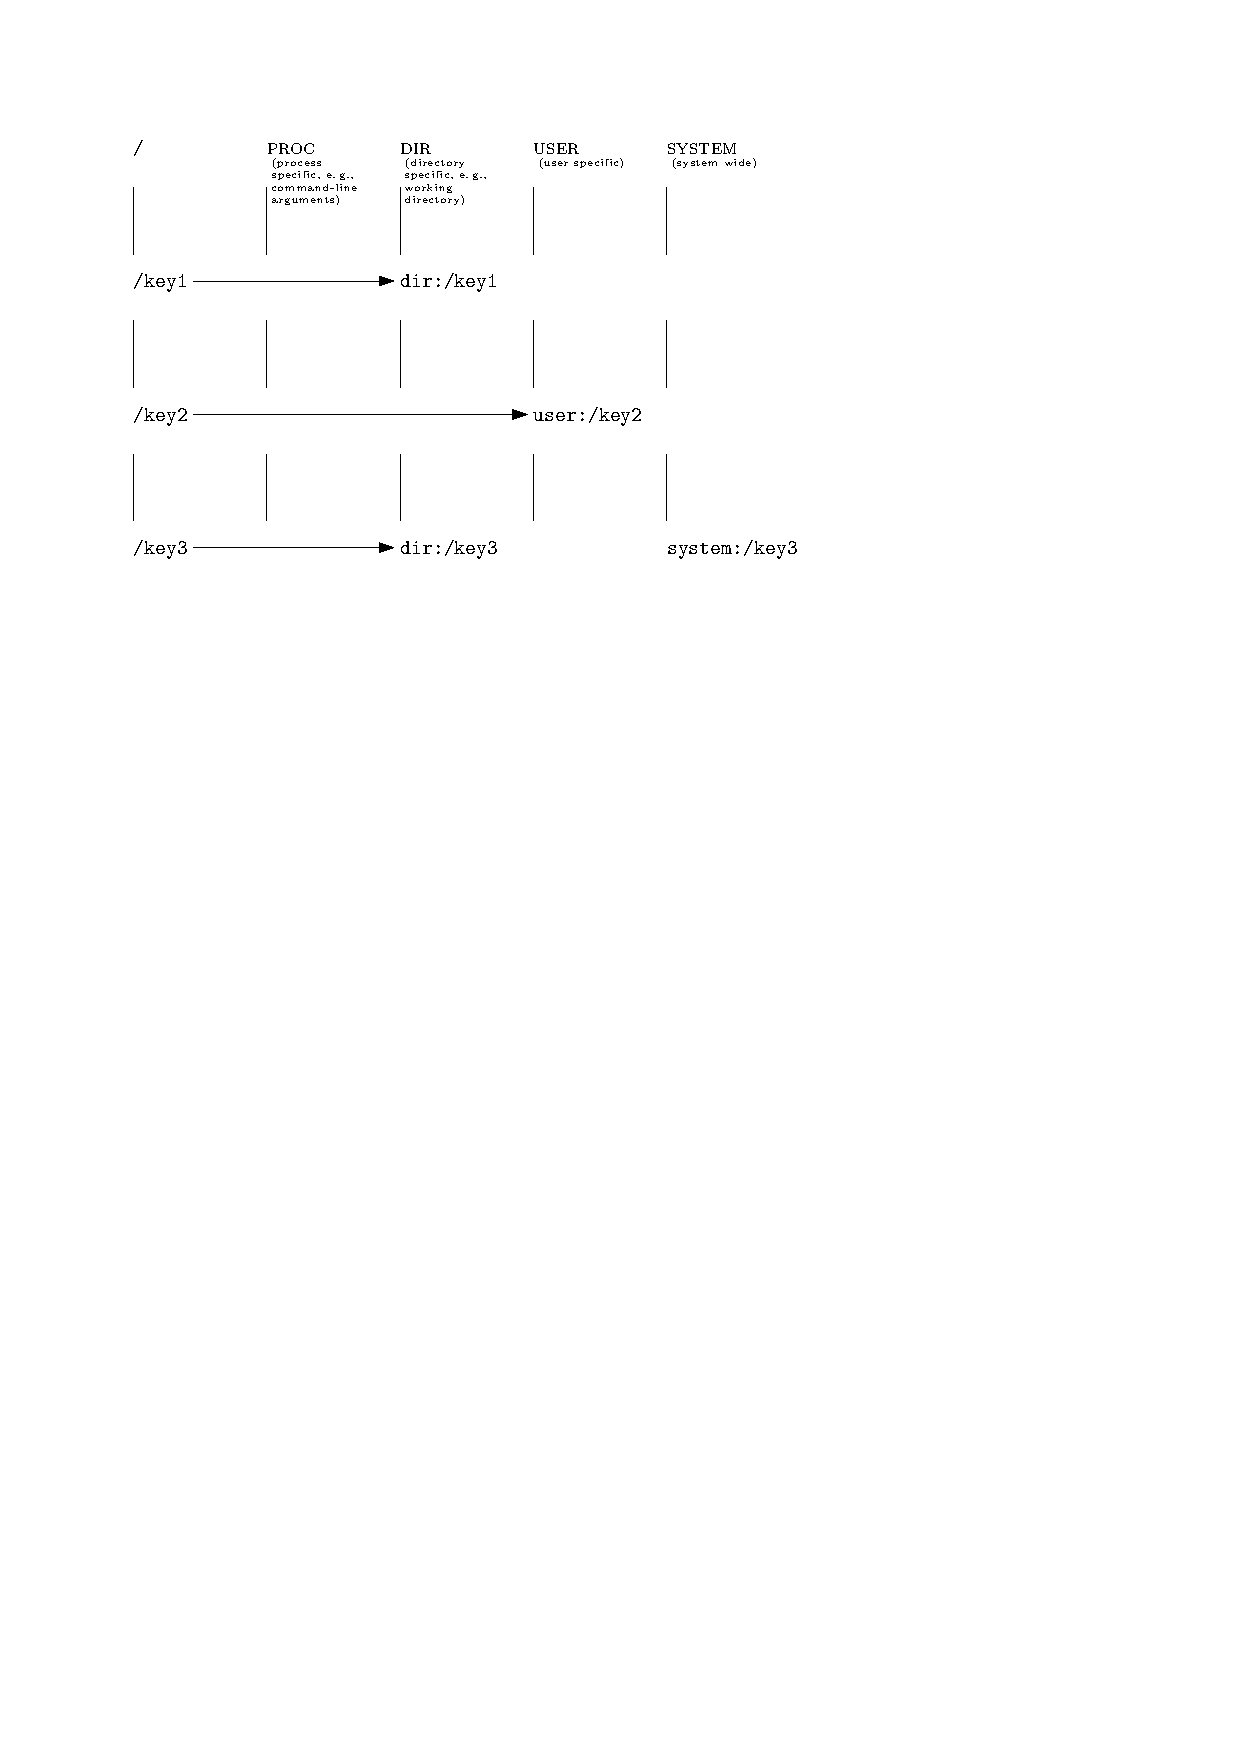
\includegraphics[scale=0.7]{cascading}
\end{frame}

\begin{frame}
	\frametitle{Contextual Values}

	\begin{task}
	What are contextual values?
	\end{task}

	\pause

	\ExecuteMetaData[../book/background.tex]{contextual-values}
\end{frame}

\begin{frame}
	\frametitle{Introspection vs.\ Code Generation (Recapitulation)}

	\begin{task}
	Advantages/Disadvantages of key database (vs.\ code generation)?
	\end{task}

	\pause

	\begin{description} %[leftmargin=0cm] %TODO: move left
	\item[$+$] specification can be updated live on the system without recompilation
	\item[$+$] tooling has generic access to all specifications
 	\item[$+$] new features the key database (e.g., better validation) are immediately available consistently
	\item[$-$] less techniques for performance improvements
	\item[$-$] contextual values cannot be used if context differs within same thread
	\end{description}

	\begin{alertblock}{Implication}
	We generally prefer introspection, except for a very thin configuration access API.
	\end{alertblock}
\end{frame}

\begin{frame}
	\frametitle{Key Databases (Recapitulation)}

	\methodQuestion{} \question{Which configuration systems/libraries/APIs have you already used or would like to use in one of your FLOSS project(s)?}

	\pause

	\begin{itemize}
	\item Command-line arguments (\p{92}, $n=222$)
	\item environment variables (\p{79}, $n=218$)
	\item configuration files (\p{74}, $n=218$)
	\item Freedesktop standards (\p{20}, $n=205$)
	\item Windows Registry (\p{13}) ($\leq$ \p{13}, $n\geq185$) [talk later]
	\item X/Q/GSettings (\p{4}, \p{11}, \p{9})
	\item KConfig (\p{5})
	\item dconf (\p{7})
	\item plist (\p{7})
	\end{itemize}

\end{frame}

\begin{frame}
	\frametitle{Definition Configuration Management (Recapitulation)}

	\begin{task}
	What is Configuration Management?
	\end{task}

	\pause

	\begin{itemize}
	\item is a discipline in which configuration (in the broader sense) is administered.
	\item makes sure computers are assembled from desired parts and the correct applications are installed.
	\item has means to describe the desired configuration of the whole managed system.
	\item ensures that the execution environment of installed applications is as required.
	\end{itemize}
\end{frame}

\begin{frame}
	\frametitle{Possible Benefits of CM (Recapitulation)}

	\begin{task}
	What are the goals of Configuration Management?
	\end{task}

	\pause

	\begin{itemize} %[<+-| alert@+>]
	\item The same goals scripts have: \\
		Documentation, Customization, Reproducability
	\item Declarative description of the system \\
		Single Source of Truth 
		(Infrastructure as Code~\cite{waldemar2013testing})
	\item Auditability
	\item Less configuration drift
	\item Error handling
	\item Pull/Push
	\item Reusability
	%\item (Resource) Abstractions
	\end{itemize}
\end{frame}

\begin{frame}
	\frametitle{Types of Specifications (Recapitulation)}

	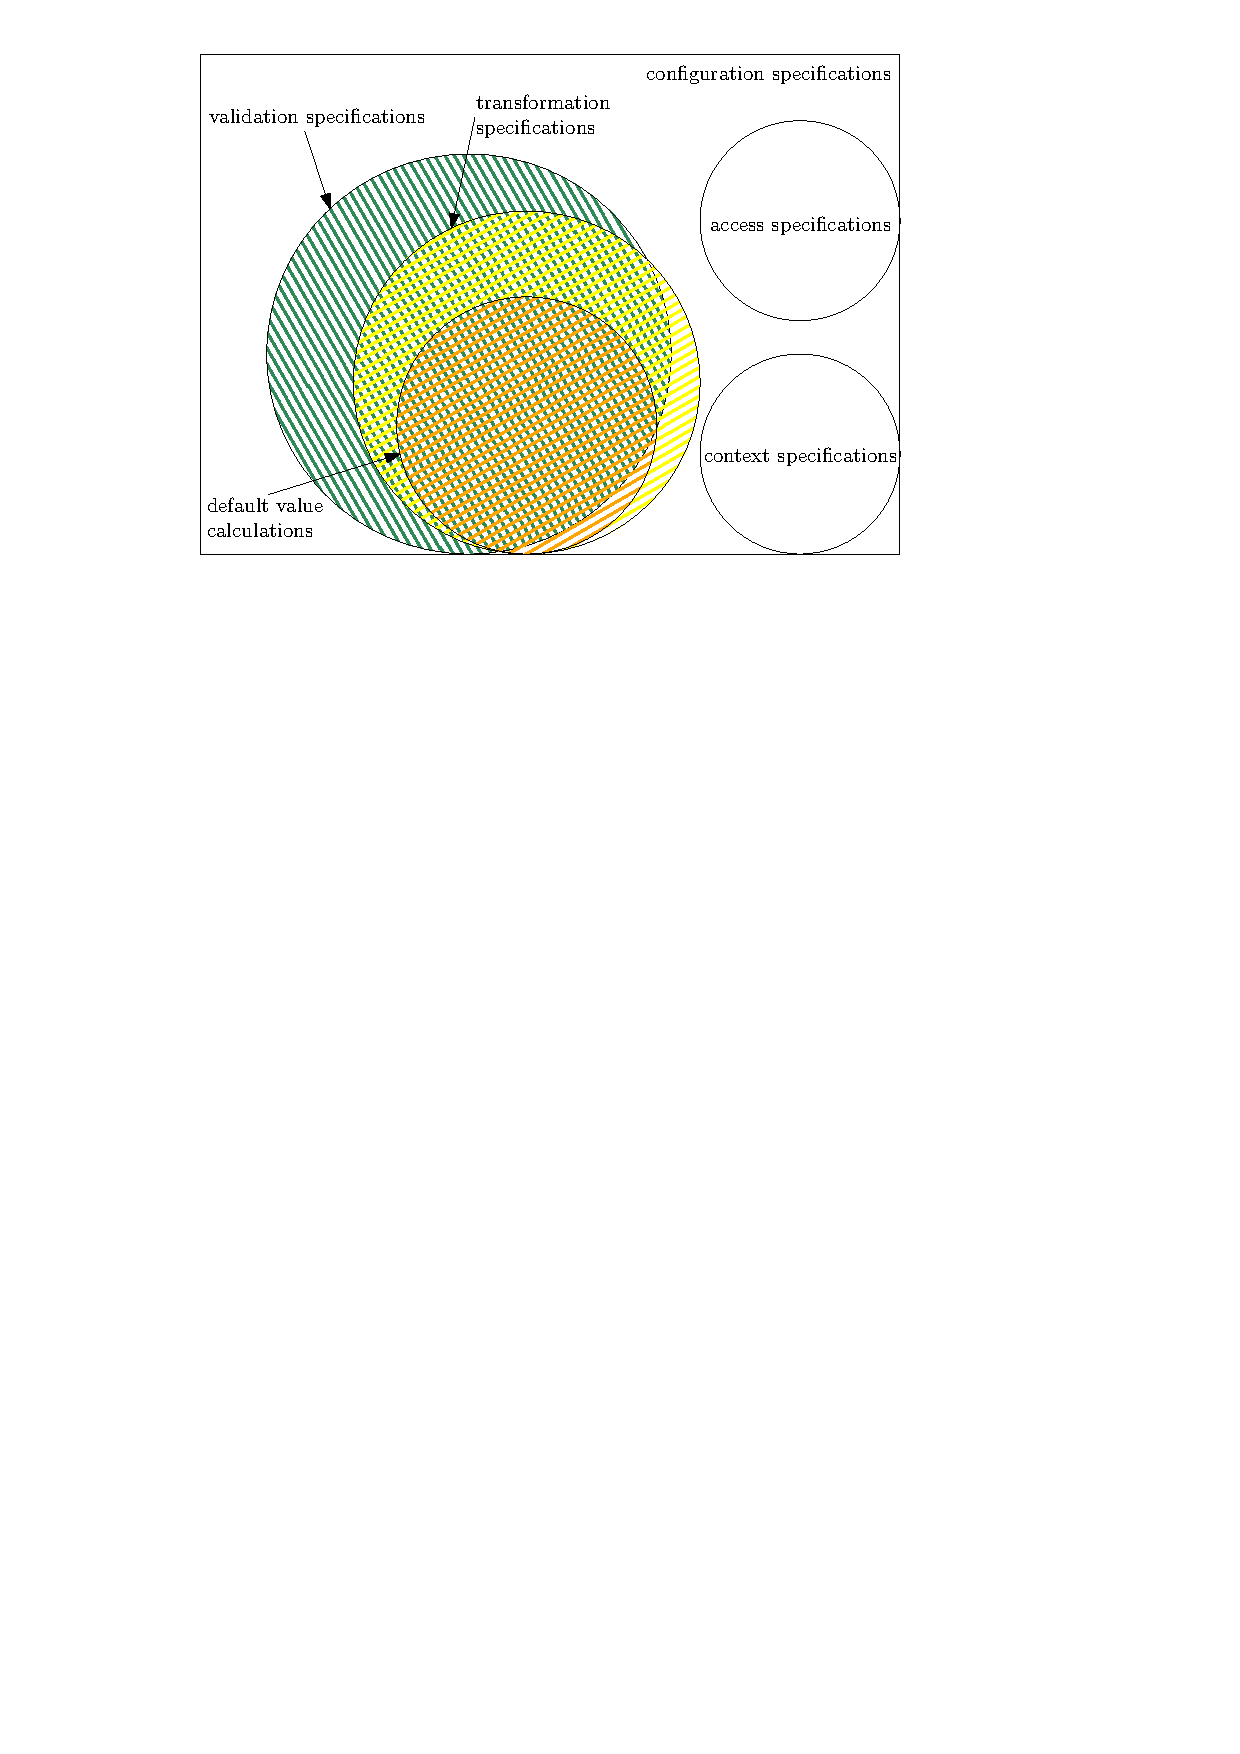
\includegraphics[scale=0.8]{specifications}
\end{frame}


\begin{frame}
	\frametitle{Configuration Specification (Partly Recapitulation)}

	\begin{task}
	How can we combine configuration specifications and configuration management?
	(Think, Pairs, Share)
	\end{task}

	\pause

	\begin{itemize}[<+-| alert@+>]
	\item configuration settings are simply an instantiation of the configuration specifications.
		Code describing the instantiation is \textbf{CM code}.
	\item configuration design is explicit (like transformations and default values) and can help while writing CM code.
	\item CM code can even be generated from the specification.
	\item access specifications make access trivial via uniform interface.
	\item visibility and similar techniques may help dealing with complexity.
	\end{itemize}
\end{frame}

\begin{frame}
	\frametitle{Configuration Drift (Recapitulation)}

	\begin{task}
	What is configuration drift? What are its causes?
	\end{task}

	\pause

	Are derivations of the ``Single Source of Truth'' (the CM code).

	Caused by:

	\begin{itemize} %[<+-| alert@+>]
	\item manual configuration changes by administrators
	\item manual configuration changes by end users
	\item differences in updates (e.g., skipped or failed updates)
	\item failed attempts to change configuration
	\item applying different versions of CM code
	\item \dots
	\end{itemize}


\end{frame}

\begin{frame}
	\frametitle{Push vs.\ Pull}

	\begin{task}
	Explain the Push and the Pull Model.
	What are their (dis)advantages?
	\end{task}

	\pause

	\begin{itemize} %[<+-| alert@+>]
	\item Push is more interactive.
	\item Push cannot do its job if nodes are not reachable.
	\item Push needs additional techniques to scale with many nodes.
	\item Push demands access to servers from a single server.
	\item Pull needs additional monitoring to know when a patch has been applied.
	\item Pull needs resources even if nothing is to do.
	\end{itemize}
\end{frame}


\begin{frame}
	\frametitle{Idempotence (Recapitulation)}

	\begin{task}
	What is idempotent, self-describing, round-tripping configuration?
	\end{task}

	\pause


	\begin{description}
	\item[Idempotent]
	yield the same configuration with any number of applications from CM code ($n\ge1$)~\cite{waldemar2013testing}:
	\[
		f(f(x))=f(x)
	\]

	\item[Self-describing]
	means that from the configuration file alone we are able to derive the correct internal representation.~\cite{wadler2003xml}

	\item[Round-tripping]
	means that if a file is serialized and then parsed again, we end up with an identical internal representation.~\cite{wadler2003xml}

	\end{description}
\end{frame}

\begin{frame}
	\frametitle{Examples}

	XML has neither of the last two property~\citet{wadler2003xml}:

	\begin{itemize}[<+-| alert@+>]
	\item internal representation crucially depends on XML schema
	\item union of integer and strings
	\end{itemize}

	\pause[\thebeamerpauses]  %  show after \begin{itemize}[<+->]

	Idempotence~\cite{waldemar2013testing}:

	\begin{itemize}[<+-| alert@+>]
	\item to guarantee repeatability
	\item 92 scripts were non-idempotent out of 298
	\item configuration overwritten by package installation
	\end{itemize}
\end{frame}

\begin{frame}
	\frametitle{Checking Configurations (Recapitulation)}

	\begin{task}
	Which properties of configuration settings can be checked?
	\end{task}

	\pause

	\begin{itemize} %[<+-| alert@+>]
	\item structure
	\item values (data types)
	\item constraints
	\item semantic checks (e.g., IP, folder)
	\item domain-specific checks (e.g., databases)
	\item requirements (suitable configurations)
	\item context (context-aware configurations)
	\end{itemize}
\end{frame}

\begin{frame}
	\frametitle{Checking Specifications}

	\begin{task}
	What are the goals of checking \elektra{Spec} are:
	\end{task}

	\pause

	\begin{itemize} %[<+-| alert@+>]
	\item Defaults must be present for safe lookups.
	This goal also implies that there must be at least one valid configuration setting.
	\item Types of default values must be compatible with the types of the keys.
	\item Every contextual interpretation of a key must yield a compatible type.
	\item Links must not refer to each other in cycles.
	\item Every link and the pointee must have compatible types.
	\end{itemize}
\end{frame}

\begin{frame}[fragile]
	\frametitle{Example (Recapitulation)}

	\begin{code}[morekeywords={override},gobble=4]
	[sw/org/abc/has_true_arg]
	  type:=boolean
	  default:=0
	  override/#0:=/sw/org/abc/arg0
	  override/#1:=/sw/org/abc/arg1
	\end{code}
\end{frame}

\begin{frame}[fragile]
	\frametitle{Logfile Extensions (Recapitulation)}

	\begin{code}[morekeywords={match,path},gobble=4]
	[slapd/logfile]
	  check/path:=file
	  check/validation:=^/var/log/
	  check/validation/message:=Policy violation:
	    log files must be below /var/log
	\end{code}
\end{frame}

\begin{frame}
	\frametitle{CM Languages (Recapitulation)}

	\begin{itemize}[<+-| alert@+>]
	\item What is the relationship to software configuration management (Proteus/PCL)?
	\item[] Build systems may provide configuration management features.
	\item How is it possible to provide referential transparency both for the configuration specification language and for the system itself (NIX)?
	\item[] By functional languages and file system (layouts).
	\item Which notations for CM exist?
	\item[] Text,  Graphical (UML), Semi-structured, Key-value, Structured
	\end{itemize}
\end{frame}

\begin{frame}
	\frametitle{Popular CMs today (Recapitulation)}

	\begin{itemize} %[<+-| alert@+>]
	\item CFengine
	%\item Bcfg2
	\item LCFG
	\item Config Mgmt
	\item Quattor
	\item Puppet
	\item Chef
	\item Ansible (Talk next week)
	\item SaltStack (Talk today)
	\item Rudder
	\item Spacewalk
	\end{itemize}
\end{frame}

\begin{frame}
	\frametitle{Elektra (Recapitulation)}

	\begin{task}
	What is Elektra?
	\end{task}

	\pause

	\begin{itemize}
	\item is not only a key database but a specification language to describe a key database
	\item plugins implement the specification (could be distributed but focus is configuration files)
	\item is library based (no single point of failure, no distributed coordination needed)
	\item supports transactions (persisting whole KeySets at once)
	\item supports integration of existing configuration
	\end{itemize}
\end{frame}



%%%%%%%%%%%%%%%%%%%%%%%%%%%%%%%%%%%%%%%%%% 
\section{Error Messages}

\subsection{}

\begin{frame}[fragile]
	\frametitle{Motivation (Recapitulation)}

	Error messages are extremely important as they are the main communication channel to system administrators.\\
	Example specification:
	\vspace{1em}

	\begin{code}[morekeywords={assign,math},gobble=4]
	[a]
	  check/type:=long
	[b]
	  check/type:=long
	[c]
	  check/range:=0-10
	  assign/math:=../a+../b
	\end{code}
\end{frame}

\begin{frame}
	\frametitle{Considerations (Recapitulation)}

	\begin{itemize}[<+-| alert@+>]
	\item Generic vs.\ specific plugins
	\item General principles of good error messages~\cite{lee2011personifying}
	\item Give context
	\item Precisely locate the cause
	\end{itemize}
\end{frame}

\begin{frame}
	\frametitle{Further Considerations}

	\begin{itemize}[<+-| alert@+>]
	\item configuration design first: avoid errors if possible
	\item should not leak internals~\cite{brown1983error}
	\item ``edit here mentality'': never point to correct statements~\cite{marceau2011mind}
	\item do not propose solutions~\cite{marceau2011mind}
	\item reduce vocabulary~\cite{marceau2011mind}
	\item precision and recall\footnote{terms from classification, it is the numerical counterpart of soundness and completeness}~\cite{wrenn2017error}
	\item tension between providing enough information and not overwhelming the user~\cite{wrenn2017error}
	\item colors might help~\cite{wrenn2017error}
	\end{itemize}
\end{frame}

\begin{frame}
	\frametitle{Error Messages for Misconfiguration~\cite{zhang2015proactive}}

	\begin{itemize}[<+-| alert@+>]
	\item error messages are often the sole data source
	\item tool uses misconfiguration injection and check if error message point to the correct setting
	\item needs system tests
	\item missing error message means the configuration specification is not complete
	\end{itemize}
\end{frame}

\begin{frame}
	\frametitle{Context for error messages}

	\begin{itemize}[<+-| alert@+>]
	\item pin-point key and value
	\item show mountpoint (to make relative keys unique)
	\item show file name and line number
	\item unclear: show module and source code lines (for debugging)
	\end{itemize}
\end{frame}

\begin{frame}[fragile]
	\frametitle{Precise Location (Recapitulation)}

	\begin{code}[language=CfgElektra,gobble=4]
	a=5  ; unmodified
	b=10 ; modification bit in metadata
	     ; is only set here
	c=15 ; unmodified by user but changed
	     ; later by assign/math
	\end{code}
\end{frame}

\begin{frame}[fragile]
	\frametitle{Example Error Messages (Recapitulation)}
\begin{verbatim}
Sorry, I was unable to change the configuration settings!
Description: I tried to set a value outside the range!
Reason: I tried to modify b to be 10 but this caused c to
        be outside of the allowed range (0-10).
Module: range
At: sourcefile.c:1234
Mountpoint: /test
Configfile: /etc/testfile.conf
\end{verbatim}
\end{frame}




%%%%%%%%%%%%%%%%%%%%%%%%%%%%%%%%%%%%%%%%%% 
\section{User View}

\subsection{}


\begin{frame}
	\frametitle{}

	\begin{itemize}[<+-| alert@+>]
	\item system administrators: the unsung heroes
	\item interest of understanding administrators emerged around 2002~\cite{anderson2002researching}.
	\item field study also done in industry \cite{barrett2004field}.
	\item Typical methods are surveys, diary studies, interviews and observations (ethnographic field study).
	\item Barrett \cite{barrett2003system} tried to initiate a workshop at CHI 2003 to draw the attention of the HCI community towards system administration.
	\item The workshop was already dropped in the next year.
	\item The tenor is that ``tools ... are not well aligned''~\cite{haber2007design}
	\end{itemize}
\end{frame}

\begin{frame}
	\frametitle{7 people, 1 command-line~\cite{barrett2004field}}

	\begin{itemize}[<+-| alert@+>]
	\item system administrator misunderstood problem (had a wrong assumption)
	\item 7 people sought attention and trust, competing to tell him what to do
	\item due to wrong assumption communicated to everyone, people could not help
	\item there were several instances in which the admin ignored or misinterpreted evidence of the real problem
	\item eventually someone else solved the problem: from/to port was switched and firewall blocked these requests
	\end{itemize}
\end{frame}

\begin{frame}
	\frametitle{other cases~\cite{barrett2004field}}

	\begin{itemize}[<+-| alert@+>]
	\item lost semicolon: execution of script failed due to missing semicolon, then they tried to delete non-existent table
	\item crontab: onltape/ofltape confused because of discussion about offline backup (although an online backup should be performed)
	\item crit sit: many system administrators tried to write simple script, they competed against each other. The crit sit continued for two weeks
	\end{itemize}
\end{frame}


\begin{frame}
	\frametitle{Haber \cite{haber2007design}}

	Later Haber \cite{haber2007design} repeated a ethnographic field study.
	The stories are similar to \cite{barrett2004field}.
	They study was also conducted in the same company.
\end{frame}



\begin{frame}
	\frametitle{Database Administrator~\cite{haber2007design}}

	\begin{itemize}[<+-| alert@+>]
	\item frequent contact via phone, e-mail and IM
	\item needs to work on weekends
	\item pair-programming for new tasks
	\item typical errors: stopping wrong database process
	\end{itemize}
\end{frame}

\begin{frame}
	\frametitle{Web Administrator~\cite{haber2007design}}

	\begin{itemize}[<+-| alert@+>]
	\item crit sit
	\item deploying new Web applications
	\item about 20-400 steps to deploy an application
	\item moving from test to production done by hand
	\end{itemize}
\end{frame}

\begin{frame}
	\frametitle{Security Administrator~\cite{haber2007design}}

	\begin{itemize}[<+-| alert@+>]
	\item Gets emails on suspicious activities
	\item multi-user chat
	\item ad-hoc scripts
	\end{itemize}
\end{frame}


\begin{frame}
	\frametitle{Haber \cite{haber2007design}}

	\begin{itemize}[<+-| alert@+>]
	\item ``if data is lost...that is when you write your resume.''
	\item \p{90} is spent with communicating with other admins
	\item \p{20} of the time is spent in diversions~\cite{barrett2004field}
	\item \p{20} of the time people communicated about \emph{how to communicate}~\cite{barrett2004field}
	\item \p{6} is gathering information and running commands
	\item quality control: monitoring found that non-functional service was down two days
	\item CLIs were generally preferred
	\item configuration and log files were scattered, poorly organized and often used inconsistent terminology
	\end{itemize}
\end{frame}


\begin{frame}
	\frametitle{design principles \cite{barrett2004field}}

	\begin{itemize}[<+-| alert@+>]
	\item syntax checking is essential
	\item replicating actions should be easy
	\item undo important
	\item do not assume a complete mental model (``if understand the system is a prerequisite [...], we are lost'')
	\item do not assume programming skills (only \p{35} reported having a bachelor's degree)
	\item trust in CLI tools but little trust in GUIs (is the information up-to-date?)
	\item errors should not lead to inconsistent state
	\end{itemize}
\end{frame}

\begin{frame}
	\frametitle{design principles \cite{haber2007design}}

	Many design principles for tools were be given~\cite{haber2007design}:

	\begin{itemize}[<+-| alert@+>]
	\item configuration and logs should be displayed in an uniform way
	\item APIs/plugins for tools should be provided
	\item errors in configuration need to be discovered quickly
	\item confusion of similar settings should be avoided: add links, explain interactions
	\item provide means of comparing configuration settings
	\item provide consistent profiles of information
	\item both transient and persistent settings should be visible
	\item when errors occur: always display which changes have been made
	\end{itemize}
\end{frame}


\begin{frame}
	\frametitle{}

	In Velasquez~\cite{velasquez2008designing} interviews and a survey were combined.
	In interviews they found out that which tools were used by administrators varied widely.
	The main part of the paper, however, was quantitative.
	The result of the study was which attributes of tool are considered as important.
\end{frame}

\begin{frame}
	\frametitle{}

	Further directions:

	\begin{itemize}[<+-| alert@+>]
	\item Is the extensive communication wanted?
	\item Is it different when using CM tools?
	\end{itemize}
\end{frame}

\begin{frame}
	\frametitle{}

	Elektra's goals are:

	\begin{itemize}[<+-| alert@+>]
	\item it should be easy to develop new tools
	\end{itemize}
\end{frame}




%%%%%%%%%%%%%%%%%%%%%%%%%%%%%%%%%%%%%%%%%% 
\nocite{raab2017introducing}

\appendix

\begin{frame}[allowframebreaks]
	\bibliographystyle{plainnat}
	\bibliography{../shared/elektra.bib}
\end{frame}

\end{document}


%TODO: add cliffhanger with preview for next time
